\documentclass[11pt,letterpaper]{article}
\usepackage[lmargin=1in,rmargin=1in,tmargin=1in,bmargin=1in]{geometry}

% -------------------
% Packages
% -------------------
\usepackage{
	amsmath,			% Math Environments
	amssymb,			% Extended Symbols
	enumerate,		    % Enumerate Environments
	graphicx,			% Include Images    
	lastpage,			% Reference Lastpage
	multicol,			% Use Multi-columns
	multirow,			% Use Multi-rows
	siunitx
}

\graphicspath{{./images/}}

\usepackage{wrapfig}

% -------------------
% Font
% -------------------
\usepackage[T1]{fontenc}
\usepackage{charter}    


% -------------------
% Heading Commands
% -------------------
\newcommand{\class}{Mu Alpha Theta}
\newcommand{\term}{2022-2023}
\newcommand{\head}[2]{%
\thispagestyle{empty}
\vspace*{-0.5in}
\noindent\begin{tabular*}{\textwidth}{l @{\extracolsep{\fill}} r @{\extracolsep{6pt}} l}
	\textbf{#1} & \textbf{Name:} & \makebox[5.75cm]{\hrulefill} \\
	\textbf{#2} & & \\
	\textbf{\class:\; \term} & & \\
\end{tabular*} \\
\rule[2ex]{\textwidth}{2pt} %
}


% -------------------
% Commands
% -------------------
\newcommand{\prob}{\noindent\textbf{Problem. }}
\newcounter{problem}
\newcommand{\problem}{
	\stepcounter{problem}%
	\noindent \textbf{Problem \theproblem. }%
}
\newcommand{\pointproblem}[1]{
	\stepcounter{problem}%
	\noindent \textbf{Problem \theproblem.} (#1 points)\,%
}
\newcommand{\pspace}{\par\vspace{\baselineskip}}
\newcommand{\ds}{\displaystyle}


% -------------------
% Header & Footer
% -------------------
\usepackage{fancyhdr}

\fancypagestyle{pages}{
	%Headers
	\fancyhead[L]{}
	\fancyhead[C]{}
	\fancyhead[R]{}
\renewcommand{\headrulewidth}{0pt}
	%Footers
	\fancyfoot[L]{}
	\fancyfoot[C]{}
	\fancyfoot[R]{}
\renewcommand{\footrulewidth}{0.0pt}
}
\headheight=0pt
\footskip=14pt

\pagestyle{pages}


% -------------------
% Content
% -------------------

\begin{document}
\head{Worksheet \#1}{Date:}

% Question 1: https://artofproblemsolving.com/wiki/index.php/2014_AMC_8_Problems/Problem_9
\begin{minipage}{\textwidth}
	\problem 

	\begin{wrapfigure}[11]{r}{0.6\textwidth}
		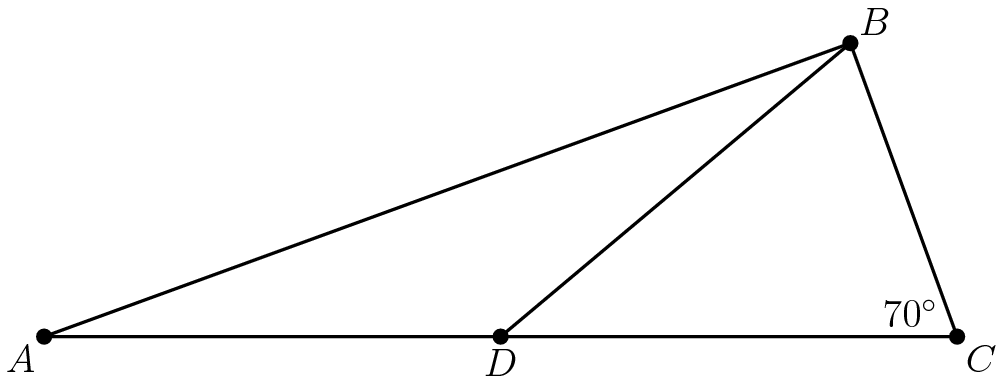
\includegraphics[width=\linewidth]{images/AMC-8-2014-P9.png}
	\end{wrapfigure}
	\noindent In $\triangle ABC$, $D$ is a point on side $\overline{AC}$ such that $BD = DC$ and $\angle BCD$ measures $\ang{70}$. What is the degree measure of $\angle ADB$? \vspace{2cm}
\end{minipage}
\vspace{8cm}

%% Question 2: https://artofproblemsolving.com/wiki/index.php/2014_AMC_8_Problems/Problem_14
\begin{minipage}{\textwidth}
	\problem

	\begin{wrapfigure}[11]{l}{0.6\textwidth}
		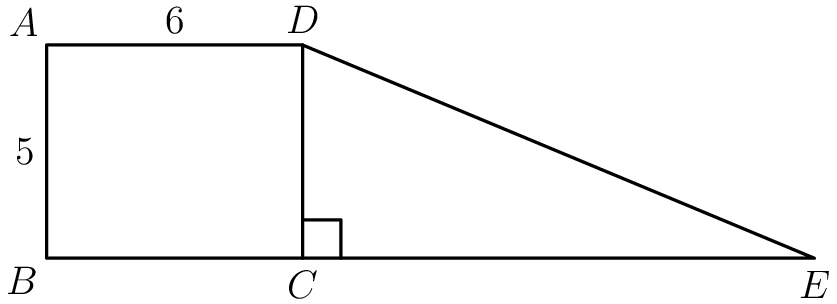
\includegraphics[width=\linewidth]{images/AMC-8-2014-P14.png}
	\end{wrapfigure}
	\noindent Rectangle $ABCD$ and right triangle $DCE$ have the same area. They are joined to form a trapezoid, as shown. What is $DE$?
\end{minipage}
\vspace{8cm}

%% Question 3: https://artofproblemsolving.com/wiki/index.php/2014_AMC_8_Problems/Problem_14
\begin{minipage}{\textwidth}
	\problem 
	\noindent A cube with $3$-inch edges is to be constructed from $27$ smaller cubes with $1$-inch edges. Twenty-one of the cubes are colored red and $6$ are colored white. If the $3$-inch cube is constructed to have the smallest possible white surface area showing, what fraction of the surface area is white?
\end{minipage}
\vspace{4cm}

%% Question 4: https://artofproblemsolving.com/wiki/index.php/2014_AMC_10B_Problems/Problem_5
\begin{minipage}{\textwidth}
	\problem 

	\noindent Doug constructs a square window using $8$ equal-size panes of glass, as shown. The ratio of the height to width for each pane is $5{\,:\,}2$, and the borders around and between the panes are $2$ inches wide. In inches, what is the side length of the square window?
	\begin{wrapfigure}[11]{l}{0.25\textwidth}
		
\includegraphics[width=\linewidth]{images/AMC-10-2014B-P4.png}
	\end{wrapfigure}
\end{minipage}
\vspace{8cm}

%% Question 5: https://artofproblemsolving.com/wiki/index.php/2014_AMC_10B_Problems/Problem_13
\begin{minipage}{\textwidth}
	\problem 

	\begin{wrapfigure}[11]{r}{0.35\textwidth}
		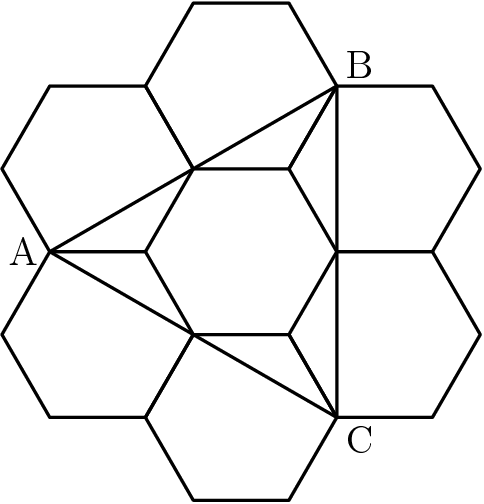
\includegraphics[width=\linewidth]{images/AMC-10-2014B-P13.png}
	\end{wrapfigure}
	\noindent Doug constructs a square window using $8$ equal-size panes of glass, as shown. The ratio of the height to width for each pane is $5{\,:\,}2$, and the borders around and between the panes are $2$ inches wide. In inches, what is the side length of the square window?
\end{minipage}
\vspace{4cm}

\end{document}			